\documentclass[12pt]{article}
\usepackage[T1]{fontenc}
\usepackage[utf8]{inputenc}
\usepackage{polski}
\usepackage{minted}
\usepackage{geometry}
\usepackage{natbib}
\usepackage{enumitem}
\usepackage{graphicx}
\usepackage{bold-extra}
\usepackage[font=small,labelfont=bf]{caption}
\usepackage{hyperref}
\usepackage{titlesec}
\usepackage{indentfirst}
\hyphenpenalty=10000
\tolerance=1000 \emergencystretch=2em
\titlelabel{\thetitle.\quad}

 \geometry{
     left=23mm,
     top=25mm,
     right=23mm
 }


\def\mydate{\leavevmode\hbox{\twodigits\day.\twodigits\month.\the\year}}
\def\twodigits#1{\ifnum#1<10 0\fi\the#1}

\begin{document}
%titlepage
\thispagestyle{empty}
\begin{center}
\begin{minipage}{0.75\linewidth}
    \centering
    
\includegraphics[width=0.45\linewidth]{agh_logo2.png}
    \par
    \vspace{2cm}
    {\bfseries{\scshape{\Huge  Teoria współbieżności}}}
    \par
    \vspace{1.7cm}
    {\scshape{\Large Laboratorium 7}}
    \par
    \vspace{0.8cm}
    {\scshape{\Large Wzorce projektowe dla}}
    \vspace{0.3cm}
    \par
    {\scshape{\Large programowania współbieżnego}}
    \par
    \vspace{3cm}

    {\scshape{\Large Albert Gierlach}}\par
    \vspace{1cm}

    {\Large \mydate}
\end{minipage}
\end{center}
\clearpage



\section{Zadanie}
Zaimplementować bufor jako aktywny obiekt (Producenci-Konsumenci).

  
\section{Koncept rozwiązania}
Na podstawie poniższego diagramu zaimplementowałem wzorzec.
\begin{center}
\centering
    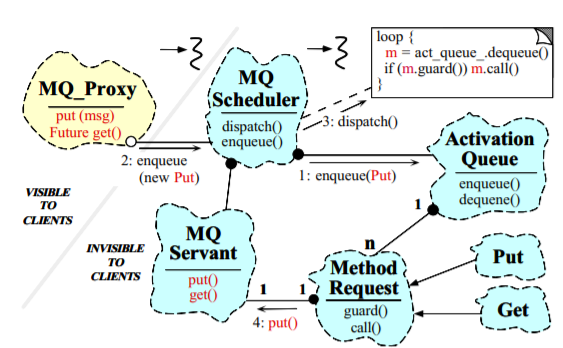
\includegraphics{active_object.png}
    \captionof{figure}{Schemat wzorca active object}
\end{center}
W przypadku problemu producentów i konsumentów, każdy z nich będzie miał do przetworzenia ustaloną liczbę elementów. Oba typy wątków wypiszą wiadomości kiedy skończą dodawanie zadań do schedulera oraz będą czekać na zakończenie zleconych operacji. Każde zadanie wypisuje swoje dane, gdy zostaje przetwarzane. Pozwoli to zaobserwować przebieg programu.


\section{Implementacja oraz wyniki}
\begin{minted}[frame=lines,
                framesep=2mm
                ]{java}
public class Servant {
    private final Queue<Integer> queue = new LinkedList<>();

    private final int capacity;

    public Servant(int capacity) {
        this.capacity = capacity;
    }

    public void put(List<Integer> data){
        queue.addAll(data);
    }

    public List<Integer> get(int elements){
        List<Integer> out = new LinkedList<>();
        while(elements-- > 0){
           out.add(queue.remove());
        }

        return out;
    }

    public int size(){
        return queue.size();
    }

    public int getCapacity() {
        return capacity;
    }
}

public interface IMethodRequest {
    void call();
    boolean guard();
}

public class AddRequest implements IMethodRequest {
    private final Servant servant;
    private final List<Integer> object;
    private final Future future;
    private final long requestingThreadID;

    public AddRequest(Future future, Servant servant, List<Integer> o) {
        this.future = future;
        this.servant = servant;
        this.object = o;
        this.requestingThreadID = Thread.currentThread().getId();
    }

    @Override
    public void call() {
        System.out.println(this);
        servant.put(object);
        future.set(List.of(object.size()));
    }

    @Override
    public boolean guard() {
        return servant.size() + object.size() <= servant.getCapacity();
    }

    @Override
    public String toString() {
        return "AddRequest by " +
                requestingThreadID +
                " - " +
                object.size() +
                " items";
    }
}

public class GetRequest implements IMethodRequest {
    private final Future future;
    private final Servant servant;
    private final int elements;
    private final long requestingThreadID;

    public GetRequest(Future future, Servant servant, int elements) {
        this.servant = servant;
        this.future = future;
        this.elements = elements;
        this.requestingThreadID = Thread.currentThread().getId();
    }

    @Override
    public void call() {
        System.out.println(this);
        future.set(servant.get(elements));
    }

    @Override
    public boolean guard() {
        return servant.size() >= elements;
    }

    @Override
    public String toString() {
        return "GetRequest by " +
                requestingThreadID +
                " - " +
                elements +
                " items";
    }
}

public class Scheduler extends Thread{
    private final Queue<IMethodRequest> activationQueue = new ConcurrentLinkedQueue<>();

    public void insert(IMethodRequest methodRequest){
        activationQueue.add(methodRequest);
    }

    @Override
    public void run(){
        while(true){
            var item = activationQueue.poll();
            if (item != null) {
                if (item.guard()) {
                    item.call();
                }else{
                    activationQueue.add(item);
                }
            }
        }
    }
}

public class Future {
    private List<Integer> object;
    private boolean done = false;

    public List<Integer> get() {
        return object;
    }

    public void set(List<Integer> o) {
        object = o;
        complete();
    }

    public synchronized void complete(){
        done = true;
        notify();
    }

    public boolean isCompleted(){
        return done;
    }

    public synchronized void await(){
        while(!isCompleted()){
            try {
                wait();
            } catch (InterruptedException ignored) {
            }
        }
    }
}

public class BufferProxy {
    private final Servant servant;
    private final Scheduler scheduler = new Scheduler();

    public BufferProxy(int bufferSize) {
        this.servant = new Servant(bufferSize);

        scheduler.setDaemon(true);
        scheduler.start();
    }

    public Future put(List<Integer> o) {
        var future = new Future();
        scheduler.insert(new AddRequest(future, servant, o));
        return future;
    }

    public Future get(int numberOfElements) {
        var future = new Future();
        scheduler.insert(new GetRequest(future, servant, numberOfElements));
        return future;
    }
}

public class Consumer extends Thread {
    private final BufferProxy proxy;
    private final int totalNumberToGet;

    public Consumer(BufferProxy proxy, int totalNumberToGet) {
        this.proxy = proxy;
        this.totalNumberToGet = totalNumberToGet;
    }

    public void _sleep(int milis){
        try{
            sleep(milis);
        }catch (InterruptedException ignored){
        }
    }

    @Override
    public void run(){
        long id = Thread.currentThread().getId();

        List<Future> futureList = new LinkedList<>();
        int elementsLeft = totalNumberToGet;
        var random = ThreadLocalRandom.current();
        while(elementsLeft > 0) {
            int toGet = Math.min(elementsLeft, random.nextInt(5) + 1);
            elementsLeft -= toGet;

            var future = proxy.get(toGet);
            futureList.add(future);

            _sleep(100);
        }

        System.out.println("Consumer " + id + " finished requesting!");
        for(var f : futureList){
            f.await();
        }
        System.out.println("Consumer " + id + " finished job!");
    }
}

public class Producer extends Thread {
    private final BufferProxy proxy;
    private final int totalNumberToPut;
    private ThreadLocalRandom random;

    public Producer(BufferProxy proxy, int totalNumberToGet) {
        this.proxy = proxy;
        this.totalNumberToPut = totalNumberToGet;
    }

    public void _sleep(int milis){
        try{
            sleep(milis);
        }catch (InterruptedException ignored){
        }
    }

    public List<Integer> generateData(int elems){
        List<Integer> out = new LinkedList<>();
        while(elems > 0){
            out.add(random.nextInt(100));
            elems--;
        }
        return out;
    }

    @Override
    public void run(){
        random = ThreadLocalRandom.current();
        long id = Thread.currentThread().getId();

        List<Future> futureList = new LinkedList<>();
        int elementsLeft = totalNumberToPut;
        while(elementsLeft > 0) {
            int toPut = Math.min(elementsLeft, random.nextInt(5) + 1);
            elementsLeft -= toPut;

            var future = proxy.put(generateData(toPut));
            futureList.add(future);

            _sleep(200);
        }

        System.out.println("Producer " + id + " finished requesting!");
        for(var f : futureList){
            f.await();
        }
        System.out.println("Producer " + id + " finished job!");
    }
}

public class Main {
    private static final int BUFFER_CAPACITY = 10;
    private static final int CONSUMER_THREADS = 5;
    private static final int PRODUCER_THREADS = 5;
    private static final int ELEMENTS_PER_THREAD = 20;

    public static void main(String[] args) {
        var threadList = new LinkedList<Thread>();
        var bufferProxy = new BufferProxy(BUFFER_CAPACITY);

        IntStream.range(0, CONSUMER_THREADS).forEach(i -> {
            threadList.add(new Consumer(bufferProxy, ELEMENTS_PER_THREAD));
        });

        IntStream.range(0, PRODUCER_THREADS).forEach(i -> {
            threadList.add(new Producer(bufferProxy, ELEMENTS_PER_THREAD));
        });

        threadList.forEach(Thread::start);

        threadList.forEach(t -> {
            try {
                t.join();
            } catch (InterruptedException e) {
                e.printStackTrace();
            }
        });
    }
}



\end{minted}

\noindent
Wykonanie programu dało następujące wyniki:
\begin{minted}[frame=lines,
                framesep=2mm
                ]{text}
AddRequest by 23 - 4 items
GetRequest by 17 - 4 items
AddRequest by 24 - 4 items
AddRequest by 25 - 1 items
AddRequest by 22 - 4 items
GetRequest by 16 - 5 items
AddRequest by 21 - 1 items
GetRequest by 18 - 3 items
GetRequest by 20 - 1 items
AddRequest by 21 - 2 items
GetRequest by 18 - 3 items
AddRequest by 23 - 4 items
GetRequest by 16 - 3 items
AddRequest by 22 - 1 items
AddRequest by 24 - 5 items
GetRequest by 20 - 1 items
GetRequest by 19 - 4 items
GetRequest by 20 - 2 items
AddRequest by 25 - 5 items
GetRequest by 19 - 3 items
GetRequest by 19 - 2 items
AddRequest by 21 - 3 items
GetRequest by 17 - 1 items
GetRequest by 18 - 1 items
AddRequest by 25 - 1 items
AddRequest by 23 - 2 items
AddRequest by 24 - 2 items
AddRequest by 22 - 4 items
GetRequest by 17 - 4 items
GetRequest by 16 - 5 items
GetRequest by 18 - 1 items
AddRequest by 23 - 2 items
GetRequest by 20 - 1 items
GetRequest by 19 - 1 items
AddRequest by 25 - 4 items
AddRequest by 24 - 3 items
AddRequest by 21 - 1 items
GetRequest by 20 - 1 items
AddRequest by 22 - 1 items
GetRequest by 17 - 4 items
GetRequest by 18 - 2 items
GetRequest by 16 - 1 items
GetRequest by 19 - 1 items
Consumer 16 finished requesting!
Consumer 17 finished requesting!
Consumer 19 finished requesting!
AddRequest by 23 - 2 items
GetRequest by 16 - 2 items
AddRequest by 24 - 2 items
GetRequest by 20 - 1 items
GetRequest by 17 - 1 items
AddRequest by 25 - 4 items
AddRequest by 21 - 5 items
GetRequest by 18 - 2 items
AddRequest by 22 - 3 items
GetRequest by 16 - 4 items
GetRequest by 20 - 4 items
GetRequest by 17 - 2 items
Consumer 16 finished job!
Consumer 18 finished requesting!
AddRequest by 23 - 3 items
GetRequest by 20 - 3 items
Consumer 20 finished requesting!
AddRequest by 24 - 3 items
GetRequest by 20 - 2 items
AddRequest by 25 - 3 items
GetRequest by 18 - 2 items
GetRequest by 18 - 2 items
AddRequest by 21 - 1 items
AddRequest by 22 - 2 items
AddRequest by 23 - 3 items
GetRequest by 20 - 4 items
Consumer 20 finished job!
AddRequest by 25 - 2 items
GetRequest by 18 - 4 items
AddRequest by 24 - 1 items
Consumer 18 finished job!
AddRequest by 21 - 2 items
AddRequest by 22 - 4 items
GetRequest by 19 - 4 items
Producer 23 finished requesting!
Producer 23 finished job!
Producer 24 finished requesting!
Producer 25 finished requesting!
AddRequest by 21 - 1 items
Producer 25 finished job!
Producer 24 finished job!
GetRequest by 17 - 4 items
Consumer 17 finished job!
AddRequest by 22 - 1 items
AddRequest by 21 - 2 items
Producer 22 finished requesting!
Producer 22 finished job!
AddRequest by 21 - 1 items
AddRequest by 21 - 1 items
GetRequest by 19 - 5 items
Consumer 19 finished job!
Producer 21 finished requesting!
Producer 21 finished job!
\end{minted}



\section{Wnioski}
Analizując powyższy log programu można zauważyć, że działa on prawidłowo. Każdy z wątków dodaje swoje zlecenia do kolejki schedulera, a ten na podstawie warunków związanych z danym zleceniem wykonuje kolejne zadania. Operacje, które nie mogą być wykonane (np. bufor jest pełny) zostają dodane na koniec kolejki. \\

\emph{Active Object} pozwala na oddzielenie procesu wywoływania metody od jej wykonania (ponieważ wykonanie odbywa się w osobnym wątku), dzięki czemu wątek zlecający może kontynuować swoją pracę bez czekania na wynik. Zlecenia są realizowane przez planistę (\emph{Scheduler}), który może być zaimplementowany na wiele sposobów, np. za pomocą struktury FIFO lub poprzez nadawanie priorytetów poszczególnym zadaniom, dzięki czemu możemy priorytetyzować poszczególne zadania. Warto dodać, że dzięki temu znacznie upraszcza się rola programisty - nie musi on dbać o synchronizację, ponieważ zapewnia to architektura wzorca, a rozszerzenie funkcjonalności współdzielonego obiektu sprowadza się do dodania metod w klasach \emph{Proxy} oraz \emph{Servant} oraz dodaniu nowej klasy obsługującej \emph{MethodRequest}. \\

Wzorzec ten jest szeroko wykorzystywany w systemie Android, ponieważ większość aplikacji posiada wątek interfejsu graficznego (UI). Zastosowanie Active Object pozwala więc na wykonywanie obliczeń asynchronicznie, dzięki czemu interfejs aplikacji pozostaje responsywny, a gdy obliczenia w wątku schedulera się zakończą, widok zostaje uaktualniony. \\

Wadą takiego rozwiązania jest narzut dodatkowych operacji, ponieważ stosuje ono zewnętrzne mechanizmy, które przetwarzają dane, przez co wywołanie konkretnej metody nieco się przedłuża. Kolejną wadą może być trudność w debugowaniu programu, gdyż jest on wielowątkowy, a planista może szeregować zadania w różnej kolejności.



\newpage
\section{Bibliografia}
\begin{itemize}
    \item \url{https://pl.wikipedia.org/wiki/Active_object}
    \item \url{http://www.diranieh.com/DP/POSA_ActiveObject.htm}
    \item \url{https://www.dre.vanderbilt.edu/~schmidt/PDF/Act-Obj.pdf}
    \item \url{https://www.youtube.com/watch?v=U9Tf7h-etl0}
    \item \url{https://madhuraoakblog.wordpress.com/2014/05/10/active-object-pattern/}


\end{itemize}

\end{document}
